% ---------------------------------------------------------
% Project: PhD KAPPA
% File: results.2.tex
% Author: Andrea Discacciati
%
% Purpose: Paper 2 (results)
% ---------------------------------------------------------

\section{Paper II}

In \citetalias{bellavia_using_2015} we proposed the use of Laplace regression to estimate percentiles of attained age at the time of the event of interest. We also discussed the consequences in the interpretation of the survival curve in the presence of delayed entries.  %This introduces the problem of defining analysis time, and in particular the origin of the time scale. 

\subsection{Estimating percentiles of attained age at the event}

\subsubsection{Defining the time scale}
An important consideration when analyzing the distribution of survival time is the choice of the time scale. In particular, the difference between the origin of the time scale --- that is, that point in time when the subjects become at risk of experiencing the event of interest --- and the time at which subjects start to be actually followed-up merits particular attention. 

In randomized experimental studies, for example, subjects are typically considered to become at risk at the time of their random allocation to either the treatment or placebo arm. In such cases, the most natural time scale is `time since randomization' (or `follow-up time'), which takes value 0 at randomization. Given this sampling design, sometimes called `sampling the inflow', the start of the observation period coincides with the time at which individuals become at risk.

In observational epidemiologic studies, on the other hand, attained age is often a more natural time scale as compared with time since some arbitrary baseline event \citep{korn_timetoevent_1997, thiebaut_choice_2004, cologne_proportional_2012}. In this case, the time at which individuals become at risk  does not necessarily coincide with the start of the observation period. This situation is referred to as `delayed entry' --- that is, individuals become at risk before entering the study. Delayed entries introduce left-truncation, which means that some subjects are excluded from the study because they either died or experienced the event before observation began (\citealp[section~16.2]{harrell_regression_2001}; \citealp[part~VII]{rabe-hesketh_multilevel_2012}). As a result, an extra piece of information,  $T_{\textrm{entry},i}$, has to be added next to $Y_i=\min(T_i,C_i)$ and $d_i$ in order to be able to describe the survival experience of the $i$-th individual. %As for censoring, we will make the assumption that $T_{i}\perp(T_{\textrm{trunc},i}, C_i)|\mathbf{x}_i$. %TODO: not sure? why independence if you condition. 

In the specific case of COSM and prostate cancer, age is arguably a more meaningful time scale than time since baseline, which corresponds to the time when participants returned the self-administered questionnaire. As a consequence, describing the distribution of age at first diagnosis seems more natural than describing the distribution of time elapsed between baseline and diagnosis. 

Figure \ref{fig:survivalexperience} (panel A and B) exhibits the consequences of changing the time scale to the survival experience of 10 random subjects from the COSM. In particular, in panel A the time scale was follow-up time. Here, the beginning of the observation period coincided with the time men were considered to become at risk (baseline, or 1 January 1998, or `time 0'). On the other hand, in panel B the time scale for the same 10 individuals was changed to attained age, which introduced delayed entries.

\begin{figure}[ht]
\centering
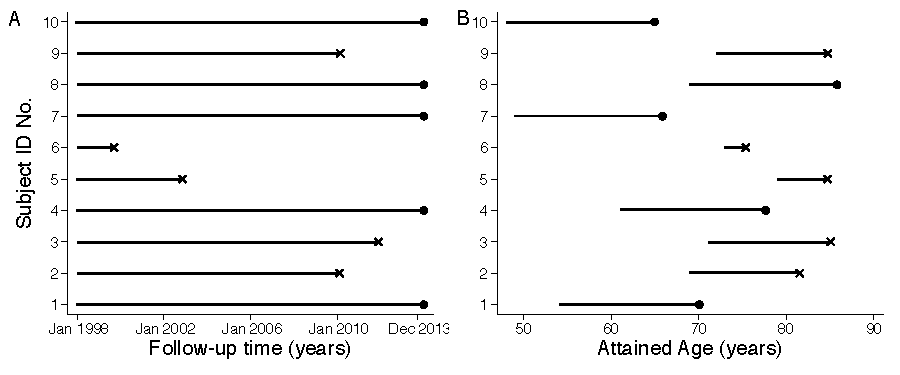
\includegraphics[width=\linewidth]{figures/survivalexperience.pdf}
\caption[Consequences of changing the primary time scale from follow-up time to attained age]{Consequences of changing the primary time scale in a prospective cohort study from follow-up time to attained age. Panels A and B illustrate the observation period for a subset of 10 participants followed up until prostate cancer diagnosis (cross) or censoring (dot).}
\label{fig:survivalexperience}
\end{figure}


\subsubsection{Consequences of delayed entries on the hazard and survival functions}
The advantage of working with the hazard function is that it is not affected by delayed entries  --- that is, by conditioning on survival until a given $t_{\textrm{entry}}$. This is, of course, because the hazard $h(t)$ is already conditioned on being event-free at time $t$ [equation (\ref{eq:hazardrate})], and therefore it makes no difference to additionally condition on survival until $t_{\textrm{entry}}<t$. As a consequence, the interpretation of the hazard function does not change.

%TODO: one sentence on likelohood PH models? See p 773 Skrondal. 

The survival function on the other hand, given its unconditional nature, is impacted by the change in the time scale. Because of the presence of delayed entries, the survival function is no longer estimating $S(t)$, but rather $S(t)/S(t_{\min})=S(t|t_{\min}$), where $t_{\min}=\min(t_{\textrm{entry},1},\ldots,t_{\textrm{entry},n})$ is the earliest entry time (\citealp[section~3.5.1]{lawless_statistical_2003}; \citealp[section~8.2.3]{cleves_introduction_2010}; \citealp{mackenzie_survival_2012}). Despite this, the interpretation of the survival curve, and in particular of the survival percentiles, remains difficult. In fact, it is no longer true that the $100p$-th survival percentile obtained from the survival curve  --- as illustrared in figure \ref{fig:kmpercentile} --- corresponds to the age by which $100p\%$ of the study population has experienced the event of interest. 

For example, figure \ref{fig:timescale} shows the survival curves for prostate cancer incidence in the COSM over the period 1998--2012 by county of enrollment, using age as the time scale. The survival curves were obtained from a flexible hazard model using equation (\ref{eq:tvphmodelssurv}). Due to delayed entries introduced by choosing attained age as the time scale, 65 years of age cannot be interpreted as the age by which 5\% of the men recruited in the Västmanland county developed prostate cancer. As an extreme example of why this is so, think that less than 5\% of the study participants from Västmanland county might have in theory entered the COSM study by 65 years of attained age.

\begin{figure}[ht]
\centering
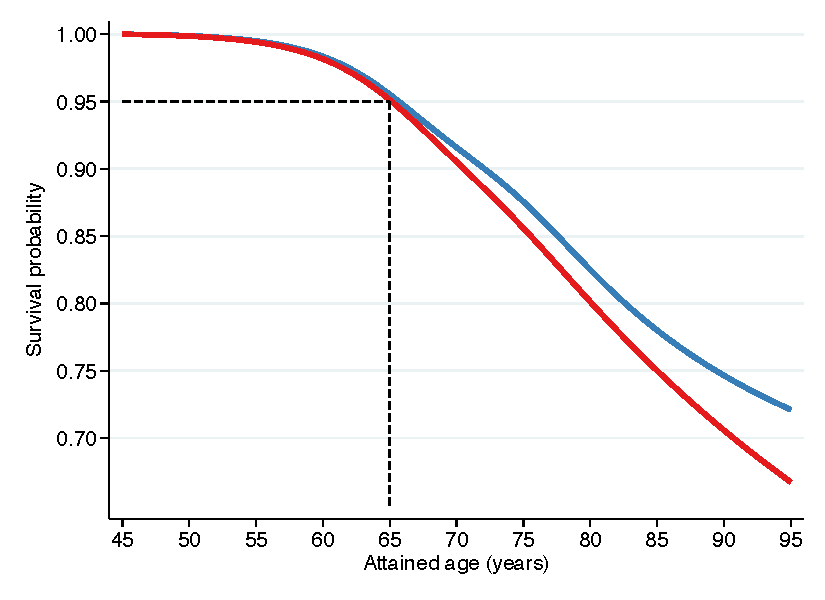
\includegraphics[width=.8\linewidth]{figures/timescale.pdf}
\caption[Survival curves for prostate cancer incidence in the COSM (1998--2012) by county of enrollment using age as the time scale]{Survival curves for prostate cancer incidence in the COSM by county of enrollment, using attained age as the time scale. Survival curves were obtained from a flexible hazard model with a time-dependent coefficient for the enrollment county variable. Baseline hazard was modeled using RCS with 5 knots. The red line refers to Västmanland county, while the blue line refers to Örebro county.}
\label{fig:timescale}
\end{figure}


%TODO: write that if the youngest dies before the next young enters than the survival curve is screwed up?

An intuitive way to circumvent this issue, and to obtain survival percentiles that are directly interpretable, is to condition the survival curve on the unique entry times (baseline ages, in our case). By doing so, the  $100p$-th survival percentile of age at the event can be interpreted as the age by which $100p\%$ of the subjects have experienced the event, conditional on a given baseline age.

\subsubsection{Use of quantile regression to model and predict percentiles of attained age at the event}

Modeling and predicting survival percentiles of age at the event, conditionally on age at baseline, is straightforward with quantile regression for censored data. This can be done through the following model:
\begin{equation}
Q_{A_i}(p|\textrm{ageBaseline}_i) = \beta_0(p) + \sum_{r=1}^b \beta_r(p)g_r(\textrm{ageBaseline}_i),
\label{eq:quantileage}
\end{equation}
where $A_i$ is age at the event and $\textrm{ageBaseline}_i$ is the baseline age for the $i$-th individual --- that is, the individual's entry time.  

Age at baseline can be modeled using $b$ flexible transformations, such as RCS or fractional polynomials. Conversely, $b=1$ and $g_1(\cdot)$ equal to the identity function impose a linear relationship between age at entry and the $p$-th percentile of age at the event. In this case, for diseases whose occurrence increases with age (such as prostate cancer mortality), one would generally expect to observe a positive regression coefficient $\beta_1(p)$.

Model \ref{eq:quantileage} can be easily extended to include other covariates. For example, one could include a binary variable $e_i$ in the model
\begin{equation}
Q_{A_i}(p|\textrm{ageBaseline}_i, e_i) = \beta_0(p) + \sum_{r=1}^b \beta_r(p)g_r(\textrm{ageBaseline}_i) + \beta_{b+1}(p)e_i.
\label{eq:quantileage_e}
\end{equation}

In this case, for a given $p$, $\beta_{b+1}(p)$ expresses the difference in the $100p$-th percentile of age at the event between exposed ($e_i=1$) and unexposed ($e_i=0$), conditional on age at baseline. For example, if $p=0.5$, the coefficient $\beta_{b+1}(0.5)$ estimates the differences in median age at the event, conditional on baseline age. An implicit assumption of Model \ref{eq:quantileage_e} is that the association between the covariate $e$ and the $100p$-th percentile of age at the event is constant across levels of age at baseline. This assumption can be relaxed by including in the model the necessary product terms between $g_r(\textrm{ageBaseline}_i)$ and $e_i$.

For example, let $e_i$ take value 1 for those men enrolled in Västmanland county and value 0 for those enrolled in Örebro county. Based on Model \ref{eq:quantileage_e}, the predicted 5th and 10th percentiles of age at prostate cancer diagnosis were, for 65-year-old men residing in Örebro county, equal to 71 and 76 years, respectively. The between-county difference in the 5th percentile of age at prostate cancer diagnosis was $-6$ months, while the 10th PD was $-10$ months, conditional on baseline age. A richer picture of the association between county of enrollment and percentiles of age at diagnosis is shown in figure \ref{fig:allp}.

More generally, the quantile regression model can be written as 
\begin{equation}
Q_{A_i}(p|\textrm{ageBaseline}_i, \mathbf{x}_i) = \beta_0(p) + \sum_{r=1}^b \beta_r(p)g_r(\textrm{ageBaseline}_i) + \sum_{j=1}^k \beta_{b+j}(p)x_{ij}.
\label{eq:quantileage_ex}
\end{equation}

The considerations made for model (\ref{eq:quantilemod}) apply to model (\ref{eq:quantileage_ex}) as well. In particular, the interpretation of the coefficients is appealing, as they are interpreted as differences in percentiles of attained age at the time of the event.

\begin{figure}[hb]
\centering
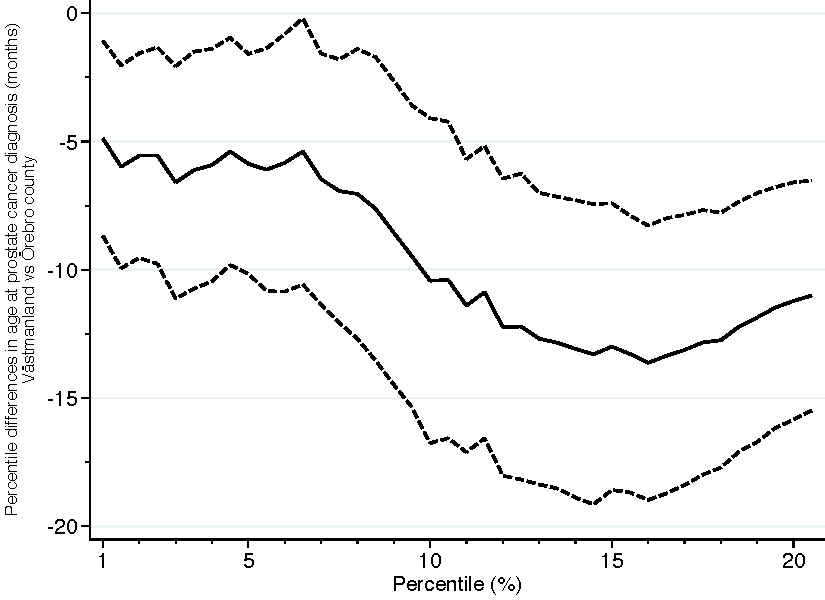
\includegraphics[width=.8\linewidth]{figures/allp.pdf}
\caption[Percentile differences in age at prostate cancer diagnosis between counties of enrollment in the COSM]{First 20 percentile differences (expressed in months) of age at prostate cancer diagnosis between men enrolled in Västmanland county and men enrolled in Örebro county, conditional on baseline age. The solid line is the point estimate, while dashed lines are 95\% confidence intervals.}
\label{fig:allp}
\end{figure}

\subsection{Body mass index and attained age at prostate cancer death}

To illustrate the use of quantile regression to model percentiles of attained age at the event, we will briefly re-analyze the updated data presented in section \ref{section:updated_paper1}. The aim is to evaluate the association between BMI and age at prostate cancer death. 

As reported in section \ref{section:updated_paper1}, BMI at baseline was modeled using RCS with 4 knots. Laplace regression was used to model the 5th percentile of age at death adjusting for total energy intake (kcal), total physical activity (MET-h/day), education (years), smoking status (current, former, never smoker), family history of prostate cancer (yes, no, don’t know), personal history of diabetes (yes, no), county of enrollment (Västmanland, Örebro), BMI at age 30 years (\kgmsq), and age at baseline (years).

For every 5-unit increment in BMI the 5th percentile of age at prostate cancer death decreased by 4 months, although the 95\% CI was observed to be quite wide ($-13$ to 5 months). No evidence of a non-linear association was observed ($p_{\textrm{non-linearity}}=0.41$). Although the magnitude of the 5th percentile difference (4 months) is not comparable with the magnitude of the MRR estimated form the Cox PH model, the directions of the associations are consistent. In particular, the negative coefficient from Laplace regression and the positive coefficient from Cox regression model (log--mortality rate ratio) indicate a worse survival, when it comes to prostate cancer mortality, among overweight and obese men as compared with lean and normal-weight men. 

Figure \ref{fig:fpc5} shows the dose--response association between BMI at baseline and differences in the 5th percentile of age at prostate cancer death.

\begin{figure}[h]
\centering
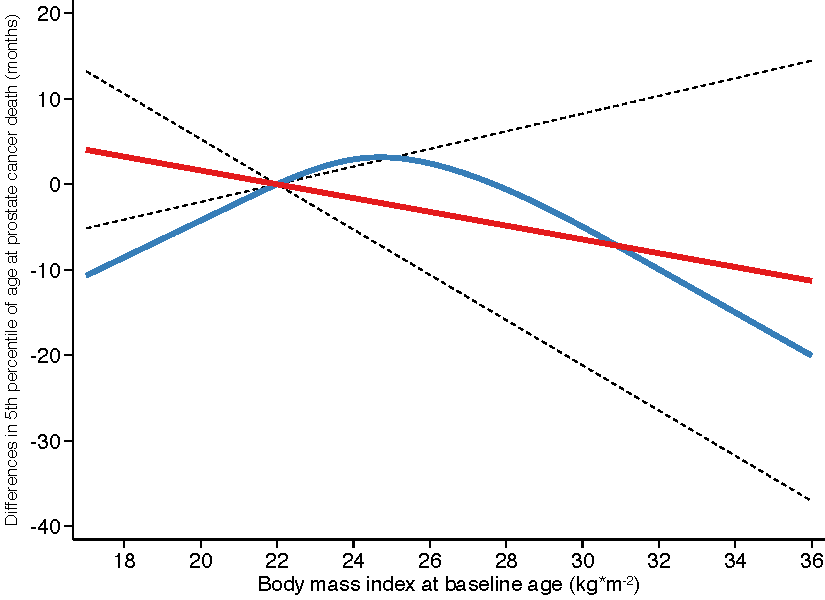
\includegraphics[width=.8\linewidth]{figures/fpc5.pdf}
\caption[Differences in the 5th percentile of age at prostate cancer death by levels of BMI at baseline]{Multivariable-adjusted differences in the 5th percentile of age at prostate cancer death by levels of BMI at baseline. BMI was modeled using RCS with 4 knots (blue line), and in a linear fashion (red line). The referent value was set at 22 \kgmsq. Black dashed lines represent the 95\% confidence interval for the linear model.}
\label{fig:fpc5}
\end{figure}

Results for the first 4 PDs in age at prostate cancer death were, for every 5-unit increment in BMI, $-2$ (95\% CI: $-14$ to 9), $-3$ (95\% CI: $-12$ to 6), $-3$ (95\% CI: $-13$ to 6), and $-4$ (95\% CI: $-14$ to 6) months. 



